% ============================================================
%  J1 — MATIN : Fondations Mathématiques & Outils Python
%  Julien Rolland — M2 Développement Fullstack
% ============================================================
\documentclass[aspectratio=169, 10pt]{beamer}
% ============================================================
%  PREAMBLE COMMUN — IA, Deep Learning & Machine Learning
%  Julien Rolland — M2 Développement Fullstack
% ============================================================

% --- Langue & encodage ---
\usepackage[utf8]{inputenc}
\usepackage[T1]{fontenc}
\usepackage{babel}
\babelprovide[import, main]{french}

% --- Thème Beamer ---
\usetheme{Madrid}
\usecolortheme{default}

% Palette de bleu académique
\definecolor{jedy_blue}{RGB}{0, 51, 102}       % bleu foncé principal
\definecolor{jedy_mid}{RGB}{0, 102, 179}        % bleu moyen accent
\definecolor{jedy_light}{RGB}{204, 221, 240}    % bleu très clair (fond boxes)
\definecolor{jedy_alert}{RGB}{180, 30, 30}      % rouge pour alertes
\definecolor{jedy_example}{RGB}{0, 120, 60}     % vert pour exemples

% Application des couleurs sur le thème Madrid
\setbeamercolor{palette primary}{bg=jedy_blue, fg=white}
\setbeamercolor{palette secondary}{bg=jedy_mid, fg=white}
\setbeamercolor{palette tertiary}{bg=jedy_blue, fg=white}
\setbeamercolor{palette quaternary}{bg=jedy_blue, fg=white}
\setbeamercolor{structure}{fg=jedy_blue}
\setbeamercolor{frametitle}{bg=jedy_blue, fg=white}
\setbeamercolor{title}{bg=jedy_blue, fg=white}
\setbeamercolor{block title}{bg=jedy_mid, fg=white}
\setbeamercolor{block body}{bg=jedy_light, fg=black}
\setbeamercolor{block title alerted}{bg=jedy_alert, fg=white}
\setbeamercolor{block body alerted}{bg=jedy_light, fg=black}
\setbeamercolor{block title example}{bg=jedy_example, fg=white}
\setbeamercolor{block body example}{bg=jedy_light, fg=black}

% --- Typographie ---
\usepackage{lmodern}
\setbeamerfont{title}{size=\Large, series=\bfseries}
\setbeamerfont{frametitle}{size=\normalsize, series=\bfseries}

% --- Navigation : suppression des icônes de navigation par défaut ---
\setbeamertemplate{navigation symbols}{}

% --- Numérotation des slides ---
\setbeamertemplate{footline}{%
  \leavevmode%
  \hbox{%
    \begin{beamercolorbox}[wd=.333\paperwidth,ht=2.25ex,dp=1ex,center]{author in head/foot}%
      \usebeamerfont{author in head/foot}\insertshortauthor
    \end{beamercolorbox}%
    \begin{beamercolorbox}[wd=.334\paperwidth,ht=2.25ex,dp=1ex,center]{title in head/foot}%
      \usebeamerfont{title in head/foot}\insertshorttitle
    \end{beamercolorbox}%
    \begin{beamercolorbox}[wd=.333\paperwidth,ht=2.25ex,dp=1ex,right]{date in head/foot}%
      \usebeamerfont{date in head/foot}
      \insertframenumber{} / \inserttotalframenumber\hspace*{2ex}
    \end{beamercolorbox}%
  }%
  \vskip0pt%
}

% --- Maths ---
\usepackage{amsmath, amssymb, amsthm}
\usepackage{bm}          % vecteurs en gras : \bm{w}

% --- Code source ---
\usepackage{listings}
\usepackage{xcolor}

\lstdefinestyle{pythonstyle}{
  language=Python,
  basicstyle=\ttfamily\footnotesize,
  keywordstyle=\color{jedy_blue}\bfseries,
  commentstyle=\color{gray}\itshape,
  stringstyle=\color{jedy_example},
  numberstyle=\tiny\color{gray},
  numbers=left,
  numbersep=5pt,
  frame=single,
  framerule=0.4pt,
  rulecolor=\color{jedy_light},
  backgroundcolor=\color{jedy_light!40},
  breaklines=true,
  showstringspaces=false,
  tabsize=4,
}
\lstset{style=pythonstyle}

% Alias pratique pour code inline
\newcommand{\code}[1]{\texttt{\small#1}}

% --- Graphiques ---
\usepackage{graphicx}
\usepackage{tikz}
\usetikzlibrary{arrows.meta, positioning, shapes.geometric, fit, calc}
\usepackage{pgfplots}
\pgfplotsset{compat=1.18}

% --- Tableaux ---
\usepackage{booktabs}
\usepackage{array}

% --- Icônes (optionnel, nécessite fontawesome5) ---
% \usepackage{fontawesome5}

% --- Macros ML/DL courantes ---
\newcommand{\R}{\mathbb{R}}
\newcommand{\E}{\mathbb{E}}
\newcommand{\Loss}{\mathcal{L}}
\newcommand{\dataset}{\mathcal{D}}
\newcommand{\X}{\mathbf{X}}
\newcommand{\y}{\mathbf{y}}
\newcommand{\w}{\mathbf{w}}
\newcommand{\W}{\mathbf{W}}
\newcommand{\grad}{\nabla}
\newcommand{\T}{^{\top}}         % transposée : \X\T
\newcommand{\lr}{\alpha}         % learning rate
\newcommand{\norm}[1]{\left\|#1\right\|}

% Encadré "Objectif pédagogique" en début de section
\newenvironment{objectif}{%
  \begin{alertblock}{Objectif}%
}{%
  \end{alertblock}%
}

% --- Infos du cours (remplacer dans chaque slides.tex) ---
\author[J. Rolland]{Julien Rolland}
\institute[Jedy]{Formation M2 Développement Fullstack}


\title[Fondations Math. \& Outils Python]{Fondations Mathématiques \& Outils Python}
\subtitle{Jour 1 — Matin}
\date{Jour 1}

% ============================================================
\begin{document}
% ============================================================

\begin{frame}
  \titlepage
\end{frame}

\begin{frame}{Plan du module}
  \tableofcontents
\end{frame}

% ============================================================
\section{Algèbre linéaire}
% ============================================================

\begin{frame}{Scalaires, Vecteurs, Matrices}
  \begin{columns}[T]
    \begin{column}{0.32\textwidth}
      \textbf{Scalaire} $x \in \R$\\[0.4em]
      Un nombre unique.\\[0.5em]
      \textit{Ex :} taux d'apprentissage $\lr = 0.01$
    \end{column}
    \begin{column}{0.32\textwidth}
      \textbf{Vecteur} $\bm{x} \in \R^n$\\[0.4em]
      $\bm{x} = \begin{pmatrix} x_1 \\ x_2 \\ \vdots \\ x_n \end{pmatrix}$\\[0.5em]
      \textit{Ex :} features d'un exemple.
    \end{column}
    \begin{column}{0.32\textwidth}
      \textbf{Matrice} $\X \in \R^{m \times n}$\\[0.4em]
      $\X = \begin{pmatrix}
        x_{11} & \cdots & x_{1n} \\
        \vdots & \ddots & \vdots \\
        x_{m1} & \cdots & x_{mn}
      \end{pmatrix}$\\[0.5em]
      \textit{Ex :} dataset ($m$ exemples, $n$ features).
    \end{column}
  \end{columns}

  \bigskip
  \begin{alertblock}{Convention de notation}
    Scalaires : $x$ (italique minuscule) \quad
    Vecteurs : $\bm{x}$ (gras minuscule) \quad
    Matrices : $\X$ (gras majuscule)
  \end{alertblock}
\end{frame}

% ---

\begin{frame}{Opérations fondamentales}
  \begin{columns}[T]
    \begin{column}{0.48\textwidth}
      \textbf{Produit scalaire} $\langle \bm{u}, \bm{v} \rangle$
      \[
        \bm{u} \cdot \bm{v} = \sum_{i=1}^{n} u_i v_i = \bm{u}\T \bm{v}
      \]
      \textit{Mesure de similarité / projection.}

      \bigskip
      \textbf{Norme euclidienne}
      \[
        \norm{\bm{x}} = \sqrt{\bm{x}\T\bm{x}} = \sqrt{\sum_i x_i^2}
      \]
    \end{column}
    \begin{column}{0.48\textwidth}
      \textbf{Produit matriciel} $\X \in \R^{m \times k}$, $\mathbf{Y} \in \R^{k \times n}$
      \[
        (\X \mathbf{Y})_{ij} = \sum_{l=1}^{k} X_{il}\, Y_{lj}
      \]
      \begin{alertblock}{Attention}
        $\X\mathbf{Y} \neq \mathbf{Y}\X$ en général !\\
        Les dimensions intérieures doivent correspondre.
      \end{alertblock}
    \end{column}
  \end{columns}
\end{frame}

% ---

\begin{frame}{Transposée \& Inverse}
  \begin{columns}[T]
    \begin{column}{0.48\textwidth}
      \textbf{Transposée} $\X\T$
      \[
        (\X\T)_{ij} = X_{ji}
      \]
      Propriété utile :
      \[
        (\X \mathbf{Y})\T = \mathbf{Y}\T \X\T
      \]
    \end{column}
    \begin{column}{0.48\textwidth}
      \textbf{Inverse} $\X^{-1}$ (matrice carrée)
      \[
        \X \X^{-1} = \X^{-1} \X = \mathbf{I}
      \]
      \begin{exampleblock}{Application directe}
        Solution du système $\X\w = \y$ :
        \[
          \w = \X^{-1}\y
        \]
        Utilisé dans la régression linéaire.
      \end{exampleblock}
    \end{column}
  \end{columns}
\end{frame}

% ---

\begin{frame}{Intuition Géométrique — Transformation Linéaire}
  \begin{columns}[T]
    \begin{column}{0.55\textwidth}
      Multiplier par une matrice \textbf{transforme l'espace} :
      \begin{itemize}
        \item \textbf{Rotation} — change l'orientation
        \item \textbf{Mise à l'échelle} — étire ou compresse
        \item \textbf{Projection} — réduit la dimension
      \end{itemize}

      \bigskip
      \begin{block}{Pourquoi ça nous importe ?}
        Un réseau de neurones = \textbf{composition} de transformations linéaires
        entrecoupées de non-linéarités.\\[0.3em]
        $\bm{h} = \sigma(\W\bm{x} + \bm{b})$
      \end{block}
    \end{column}
    \begin{column}{0.42\textwidth}
      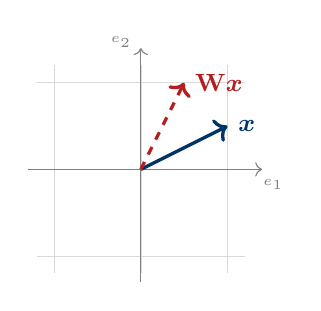
\begin{tikzpicture}[scale=1.1]
        % Grille de départ
        \draw[gray!30, very thin] (-1.2,-1.2) grid (1.2,1.2);
        \draw[->, gray] (-1.3,0) -- (1.4,0);
        \draw[->, gray] (0,-1.3) -- (0,1.4);
        % Vecteur original
        \draw[->, jedy_blue, very thick] (0,0) -- (1,0.5)
          node[right]{\small $\bm{x}$};
        % Vecteur transformé
        \draw[->, jedy_alert, very thick, dashed] (0,0) -- (0.5, 1)
          node[right]{\small $\W\bm{x}$};
        \node[below right, gray] at (1.3,0) {\tiny $e_1$};
        \node[above left, gray] at (0,1.3) {\tiny $e_2$};
      \end{tikzpicture}
    \end{column}
  \end{columns}
\end{frame}

% ============================================================
\section{Calcul différentiel}
% ============================================================

\begin{frame}{Dérivée — Taux de Variation}
  \begin{columns}[T]
    \begin{column}{0.50\textwidth}
      La dérivée mesure comment $f$ \textbf{varie localement} en $x_0$ :
      \[
        \frac{df}{dx}(x_0) = \lim_{h \to 0} \frac{f(x_0+h) - f(x_0)}{h}
      \]
      \textit{Géométriquement :} pente de la \textbf{tangente} au point $x_0$.

      \medskip
      \textbf{Dérivées usuelles :}
      \begin{center}
      {\renewcommand{\arraystretch}{1.3}%
      \begin{tabular}{ll}
        \toprule
        $f(x)$ & $\dfrac{df}{dx}$ \\[0.4em]
        \midrule
        $x^n$ & $n\,x^{n-1}$ \\
        $e^x$ & $e^x$ \\
        $\ln x$ & $1/x$ \\
        \bottomrule
      \end{tabular}}
      \end{center}

    \end{column}
    \begin{column}{0.47\textwidth}
      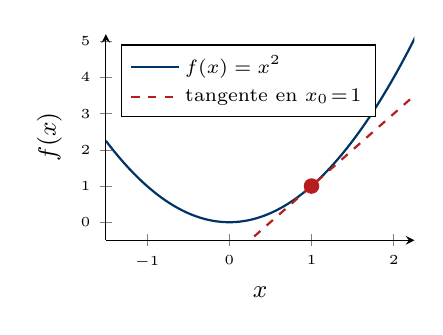
\begin{tikzpicture}
        \begin{axis}[
          width=5.5cm, height=4.2cm,
          domain=-1.5:2.3, samples=80,
          ymin=-0.5, ymax=5.2,
          axis lines=left,
          tick label style={font=\tiny},
          xlabel={\small $x$},
          ylabel={\small $f(x)$},
          xtick={-1,0,1,2},
          ytick={0,1,2,3,4,5},
          legend style={font=\scriptsize, at={(0.05,0.95)}, anchor=north west},
          legend cell align=left,
        ]
          \addplot[jedy_blue, thick] {x^2};
          \addlegendentry{$f(x)=x^2$}
          \addplot[jedy_alert, dashed, thick, domain=0.0:2.2] {2*x - 1};
          \addlegendentry{tangente en $x_0\!=\!1$}
          \addplot[only marks, mark=*,
                   mark options={fill=jedy_alert, draw=jedy_alert, scale=1.3}]
            coordinates {(1,1)};
        \end{axis}
      \end{tikzpicture}

      \smallskip
      \textbf{Règle de composition :}
      \[
        \frac{d(g \circ f)}{dx} = \frac{dg}{du} \cdot \frac{df}{dx}
        \quad (u = f(x))
      \]
    \end{column}
  \end{columns}
\end{frame}

% ---

\begin{frame}{Gradient — Extension Multivariée}
  \begin{columns}[T]
    \begin{column}{0.55\textwidth}
      Pour $f : \R^n \to \R$, le \textbf{gradient} est le vecteur des dérivées partielles :
      \[
        \nabla f(\bm{x}) =
        \begin{pmatrix}
          \dfrac{\partial f}{\partial x_1} \\[0.5em]
          \vdots \\[0.2em]
          \dfrac{\partial f}{\partial x_n}
        \end{pmatrix}
        \in \R^n
      \]

      \textbf{Exemple :} $f(x_1, x_2) = x_1^2 + x_2^2 \;\Rightarrow\;
        \nabla f = \begin{pmatrix} 2x_1 \\ 2x_2 \end{pmatrix}$

      \begin{block}{Propriété clé}
        $\nabla f(\bm{x})$ pointe dans la direction de \textbf{plus forte montée} de $f$.\\[0.3em]
        $-\nabla f(\bm{x})$ pointe donc vers la \textbf{plus forte descente}.
      \end{block}
    \end{column}
    \begin{column}{0.42\textwidth}
      \begin{center}
      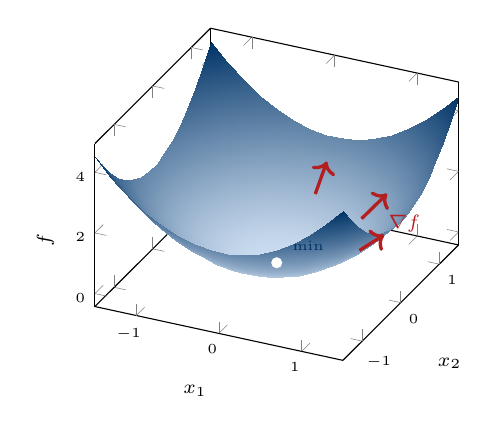
\begin{tikzpicture}
        \begin{axis}[
          width=6.2cm, height=5.8cm,
          view={25}{38},
          xlabel={\scriptsize $x_1$},
          ylabel={\scriptsize $x_2$},
          zlabel={\scriptsize $f$},
          tick label style={font=\tiny},
          label style={font=\scriptsize},
          domain=-1.5:1.5,
          y domain=-1.5:1.5,
          samples=16,
          z buffer=sort,
          colormap={jedy3d}{color=(jedy_light) color=(jedy_blue)},
          xtick={-1,0,1},
          ytick={-1,0,1},
          ztick={0,2,4},
        ]
          \addplot3[surf, shader=interp] {x^2 + y^2};
          % Flèches gradient sur la surface
          \draw[->, jedy_alert, very thick]
            (axis cs:1.00,0.00,1.00) -- (axis cs:1.30,0.00,1.69);
          \draw[->, jedy_alert, very thick]
            (axis cs:0.00,1.00,1.00) -- (axis cs:0.00,1.30,1.69);
          \draw[->, jedy_alert, very thick]
            (axis cs:0.70,0.70,0.98) -- (axis cs:0.91,0.91,1.66);
          \node[jedy_alert, font=\scriptsize]
            at (axis cs:1.45,0.20,1.90) {$\nabla f$};
          % Minimum
          \fill[white] (axis cs:0,0,0) circle (2pt);
          \node[font=\tiny, jedy_blue, above right]
            at (axis cs:0.05,0.05,0.05) {min};
        \end{axis}
      \end{tikzpicture}
      \end{center}
    \end{column}
  \end{columns}
\end{frame}

% ============================================================
\section{Probabilités (express)}
% ============================================================

\begin{frame}{Variable Aléatoire, Espérance, Variance}
  \begin{columns}[T]
    \begin{column}{0.48\textwidth}
      \textbf{Variable aléatoire} $X$\\
      Prend des valeurs selon une \textbf{distribution} $p(x)$.

      \bigskip
      \textbf{Espérance} — valeur moyenne
      \[
        \E[X] = \sum_x x\, p(x)
      \]

      \textbf{Variance} — dispersion autour de la moyenne
      \[
        \mathrm{Var}(X) = \E\left[(X - \E[X])^2\right]
      \]
    \end{column}
    \begin{column}{0.48\textwidth}
      \begin{exampleblock}{Exemple concret}
        $X$ = erreur de prédiction d'un modèle.\\[0.4em]
        $\E[X] \approx 0$ \; $\Rightarrow$ modèle non-biaisé.\\[0.4em]
        $\mathrm{Var}(X)$ faible \; $\Rightarrow$ prédictions stables.
      \end{exampleblock}

      \bigskip
      \textbf{Écart-type} $\sigma = \sqrt{\mathrm{Var}(X)}$\\[0.3em]
      Dans la même unité que $X$ — plus interprétable.
    \end{column}
  \end{columns}
\end{frame}

% ---

\begin{frame}{Distributions Utiles en ML}
  \begin{columns}[T]
    \begin{column}{0.48\textwidth}
      \textbf{Bernoulli} $X \sim \mathcal{B}(p)$
      \[
        P(X=1) = p, \quad P(X=0) = 1-p
      \]
      \textit{Utilisée pour :} classification binaire (sortie d'un neurone sigmoïde).

      \bigskip
      \textbf{Gaussienne} $X \sim \mathcal{N}(\mu, \sigma^2)$
      \[
        p(x) = \frac{1}{\sigma\sqrt{2\pi}}\,e^{-\frac{(x-\mu)^2}{2\sigma^2}}
      \]
      \textit{Utilisée pour :} initialisation des poids, bruit, régression.
    \end{column}
    \begin{column}{0.48\textwidth}
      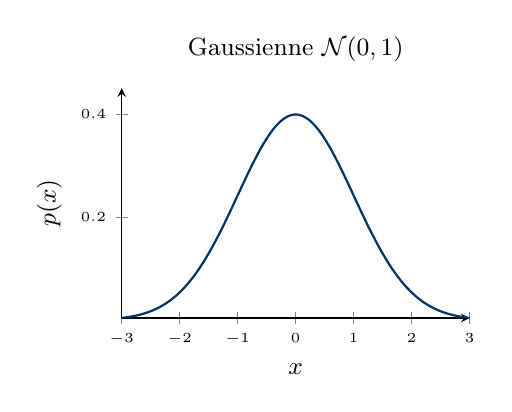
\begin{tikzpicture}
        \begin{axis}[
          width=6cm, height=4.5cm,
          xlabel={\small $x$}, ylabel={\small $p(x)$},
          xtick={-3,-2,...,3},
          ytick={0, 0.2, 0.4},
          ymax=0.45,
          tick label style={font=\tiny},
          axis lines=left,
          title={\small Gaussienne $\mathcal{N}(0,1)$},
          title style={font=\small},
        ]
          \addplot[jedy_blue, thick, domain=-3:3, samples=100]
            {exp(-x^2/2) / sqrt(2*pi)};
        \end{axis}
      \end{tikzpicture}
    \end{column}
  \end{columns}
\end{frame}

% ---

\begin{frame}{Notion de Vraisemblance}
  \begin{block}{Idée fondatrice du ML supervisé}
    On cherche les paramètres $\theta$ qui rendent les données \textbf{les plus probables} :
    \[
      \theta^* = \arg\max_{\theta}\; p(\dataset \mid \theta)
      \quad \Longleftrightarrow \quad
      \theta^* = \arg\min_{\theta}\; \Loss(\theta)
    \]
  \end{block}

  \bigskip
  \begin{columns}[T]
    \begin{column}{0.48\textwidth}
      \textbf{Log-vraisemblance} (plus pratique)
      \[
        \ell(\theta) = \log p(\dataset \mid \theta) = \sum_i \log p(y_i \mid \bm{x}_i, \theta)
      \]
      Maximiser $\ell$ = minimiser une \textbf{loss}.
    \end{column}
    \begin{column}{0.48\textwidth}
      \begin{exampleblock}{Lien avec la MSE}
        Si le bruit est gaussien, maximiser la vraisemblance revient à minimiser :
        \[
          \Loss(\theta) = \frac{1}{m}\sum_{i=1}^{m}(y_i - \hat{y}_i)^2
        \]
      \end{exampleblock}
    \end{column}
  \end{columns}
\end{frame}

% ============================================================
\section{Pourquoi Python pour l'IA ?}
% ============================================================

\begin{frame}{L'Écosystème Python IA}
  \begin{columns}[T]
    \begin{column}{0.55\textwidth}
      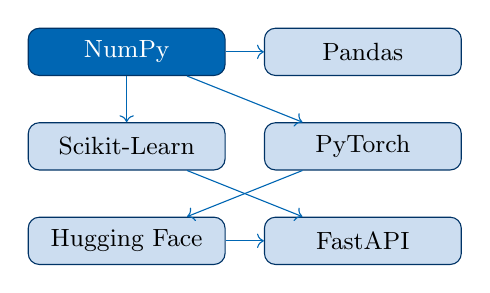
\begin{tikzpicture}[
        every node/.style={font=\small},
        box/.style={draw=jedy_blue, fill=jedy_light, rounded corners, minimum width=2.5cm, minimum height=0.6cm, align=center},
        core/.style={draw=jedy_blue, fill=jedy_mid, text=white, rounded corners, minimum width=2.5cm, minimum height=0.6cm, align=center},
      ]
        \node[core] (np) at (0,0)    {NumPy};
        \node[box]  (pd) at (3,0)    {Pandas};
        \node[box]  (sk) at (0,-1.2) {Scikit-Learn};
        \node[box]  (pt) at (3,-1.2) {PyTorch};
        \node[box]  (hf) at (0,-2.4) {Hugging Face};
        \node[box]  (fa) at (3,-2.4) {FastAPI};

        \draw[jedy_mid, ->] (np) -- (sk);
        \draw[jedy_mid, ->] (np) -- (pt);
        \draw[jedy_mid, ->] (np) -- (pd);
        \draw[jedy_mid, ->] (pt) -- (hf);
        \draw[jedy_mid, ->] (sk) -- (fa);
        \draw[jedy_mid, ->] (hf) -- (fa);
      \end{tikzpicture}
    \end{column}
    \begin{column}{0.42\textwidth}
      \textbf{Pourquoi Python ?}
      \begin{itemize}
        \item Syntaxe accessible — focus sur les idées
        \item Bibliothèques C/CUDA sous le capot\\
              $\Rightarrow$ performance native
        \item Standard de facto en recherche et industrie
      \end{itemize}

      \bigskip
      \begin{alertblock}{Ce cours}
        NumPy $\to$ Pandas $\to$ Sklearn $\to$ PyTorch $\to$ Hugging Face $\to$ FastAPI
      \end{alertblock}
    \end{column}
  \end{columns}
\end{frame}

% ---

\begin{frame}[fragile]{Jupyter Notebook — L'environnement de travail}
  \begin{columns}[T]
    \begin{column}{0.50\textwidth}
      Un notebook = \textbf{document interactif} mêlant code, résultats et texte.

      \medskip
      \textbf{Deux types de cellules :}
      \begin{itemize}
        \item \textbf{Code} — exécuté par le \textit{kernel} Python,\\
              affiche le résultat juste en dessous
        \item \textbf{Markdown} — texte formaté, formules \LaTeX,\\
              titres, explications
      \end{itemize}

      \medskip
      \begin{block}{Workflow}
        Écrire $\to$ \texttt{Shift+Enter} $\to$ voir le résultat\\
        Les variables persistent entre les cellules.
      \end{block}
    \end{column}
    \begin{column}{0.47\textwidth}
      \begin{tikzpicture}[
        cell/.style={draw=jedy_blue, rounded corners=2pt,
                     minimum width=5.2cm, minimum height=0.55cm,
                     font=\ttfamily\scriptsize, text width=5cm,
                     inner sep=4pt},
        out/.style={draw=none, font=\ttfamily\scriptsize\color{jedy_example},
                    text width=5cm, inner sep=4pt},
        lbl/.style={font=\scriptsize\bfseries, text=white,
                    fill=jedy_mid, rounded corners=1pt,
                    inner sep=2pt},
      ]
        \node[cell, fill=jedy_light]  (c1) at (0,0)
          {import numpy as np};
        \node[lbl, above left=1pt of c1.north west] {In};

        \node[cell, fill=jedy_light]  (c2) at (0,-1.0)
          {x = np.arange(5)\\print(x ** 2)};
        \node[lbl, above left=1pt of c2.north west] {In};

        \node[out] (o2) at (0,-1.9) {[ 0  1  4  9 16 ]};

        \node[cell, fill=white, draw=jedy_mid]  (c3) at (0,-2.7)
          {\# cellule Markdown\\**Résultat :** vecteur au carré};
        \node[lbl, above left=1pt of c3.north west,
              fill=jedy_example] {Md};
      \end{tikzpicture}
    \end{column}
  \end{columns}

  \begin{alertblock}{Attention — ordre d'exécution}
    Les cellules peuvent être exécutées dans n'importe quel ordre.
    Toujours relancer \textbf{Kernel $\to$ Restart \& Run All} avant de rendre un travail.
  \end{alertblock}
\end{frame}

% ---

\begin{frame}[fragile]{Le Problème des Boucles \texttt{for}}
  \begin{columns}[T]
    \begin{column}{0.48\textwidth}
      \textbf{Approche naïve Python}
\begin{lstlisting}
def dot_loop(u, v):
    result = 0.0
    for u_i, v_i in zip(u, v):
        result += u_i * v_i
    return result
\end{lstlisting}
      \begin{alertblock}{Problème}
        Python interprète chaque itération.\\
        Pour $n = 10^6$ : \textbf{\textasciitilde 200 ms}
      \end{alertblock}
    \end{column}
    \begin{column}{0.48\textwidth}
      \textbf{Approche vectorisée NumPy}
\begin{lstlisting}
import numpy as np

# Produit scalaire -- vectorise
def dot_numpy(u, v):
    return np.dot(u, v)
\end{lstlisting}
      \begin{exampleblock}{Résultat}
        Exécuté en C/BLAS.\\
        Pour $n = 10^6$ : \textbf{\textasciitilde 1 ms}\\[0.3em]
        $\approx$ \textbf{200$\times$ plus rapide}
      \end{exampleblock}
    \end{column}
  \end{columns}

  \bigskip
  \begin{block}{Règle d'or}
    En NumPy/PyTorch : \textbf{aucune boucle \texttt{for} sur les éléments}.
    Toujours chercher l'opération matricielle équivalente.
  \end{block}
\end{frame}

% ============================================================
\section{NumPy \& Vectorisation}
% ============================================================

\begin{frame}[fragile]{Anatomie d'un \texttt{ndarray}}
  \begin{columns}[T]
    \begin{column}{0.50\textwidth}
\begin{lstlisting}
import numpy as np

x = np.array([[1, 2, 3],
              [4, 5, 6]])

print(x.shape)   # (2, 3)
print(x.ndim)    # 2  <- rank
print(x.dtype)   # int64
print(x.size)    # 6
\end{lstlisting}
    \end{column}
    \begin{column}{0.46\textwidth}
      \begin{tabular}{ll}
        \toprule
        Attribut & Signification \\
        \midrule
        \code{shape}  & dimensions $(m, n, \ldots)$ \\
        \code{ndim}   & nombre d'axes (rank) \\
        \code{dtype}  & type des éléments \\
        \code{size}   & nombre total d'éléments \\
        \bottomrule
      \end{tabular}

      \bigskip
      \begin{block}{Rangs courants}
        \textbf{0D} scalaire \quad \textbf{1D} vecteur\\
        \textbf{2D} matrice \quad \textbf{3D} batch d'images
      \end{block}
    \end{column}
  \end{columns}
\end{frame}

% ---

\begin{frame}[fragile]{Slicing \& Reshape}
  \begin{columns}[T]
    \begin{column}{0.48\textwidth}
      \textbf{Slicing}
\begin{lstlisting}
X = np.arange(12).reshape(3, 4)
# [[ 0  1  2  3]
#  [ 4  5  6  7]
#  [ 8  9 10 11]]

X[0]        # 1e ligne -> [0,1,2,3]
X[:, 2]     # 3e colonne
X[1:, 1:3]  # sous-matrice
\end{lstlisting}
    \end{column}
    \begin{column}{0.48\textwidth}
      \textbf{Reshape / Vue}
\begin{lstlisting}
v = np.arange(6)       # shape (6,)
M = v.reshape(2, 3)    # shape (2,3)
F = M.flatten()        # retour (6,)

# -1 = "calcule toi-meme"
v.reshape(3, -1)       # (3, 2)
\end{lstlisting}
      \begin{alertblock}{Attention}
        \code{reshape} retourne une \textbf{vue} (pas de copie).
        Modifier la vue modifie l'original.
      \end{alertblock}
    \end{column}
  \end{columns}
\end{frame}

% ---

\begin{frame}[fragile]{Broadcasting — La Règle des Dimensions}
  \begin{columns}[T]
    \begin{column}{0.50\textwidth}
      NumPy aligne les shapes \textbf{depuis la droite}.\\
      Toute dimension de taille \textbf{1} est automatiquement étirée.

      \medskip
      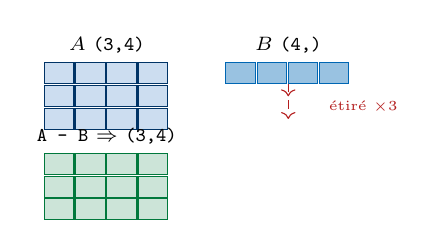
\begin{tikzpicture}[scale=0.72, every node/.style={font=\scriptsize}]
        % Matrice A (3x4)
        \foreach \r in {0,1,2} {
          \foreach \c in {0,1,2,3} {
            \draw[fill=jedy_light, draw=jedy_blue]
              (\c*0.55, -\r*0.4) rectangle ++(0.52, 0.37);
          }
        }
        \node[above] at (1.1, 0.37) {$A$ \texttt{(3,4)}};

        % Vecteur B (1x4)
        \foreach \c in {0,1,2,3} {
          \draw[fill=jedy_mid!40, draw=jedy_mid]
            (\c*0.55+3.2, 0) rectangle ++(0.52, 0.37);
        }
        \node[above] at (4.3, 0.37) {$B$ \texttt{(4,)}};

        % Flèche étirement
        \foreach \r in {1,2} {
          \draw[jedy_alert, dashed, ->] (4.3, 0) -- (4.3, -\r*0.4+0.18);
        }
        \node[right, jedy_alert] at (4.85, -0.4) {\tiny étiré $\times 3$};

        % Résultat (3x4)
        \foreach \r in {0,1,2} {
          \foreach \c in {0,1,2,3} {
            \draw[fill=jedy_example!20, draw=jedy_example]
              (\c*0.55, -\r*0.4-1.6) rectangle ++(0.52, 0.37);
          }
        }
        \node[above] at (1.1, -1.23) {\texttt{A - B} $\Rightarrow$ \texttt{(3,4)}};
      \end{tikzpicture}
    \end{column}
    \begin{column}{0.47\textwidth}
\begin{lstlisting}
X = np.random.randn(100, 5)
# shape (100, 5)

mean = X.mean(axis=0)
# shape (5,) -- une moyenne par feature

X_centered = X - mean
# (100,5) - (5,) => (100,5)
# soustrait la meme moyenne
# sur chaque ligne automatiquement

std = X.std(axis=0)
X_norm = (X - mean) / std
\end{lstlisting}
    \end{column}
  \end{columns}
\end{frame}

% ============================================================
\section{Pandas — Introduction pratique}
% ============================================================

\begin{frame}[fragile]{\texttt{DataFrame} vs \texttt{ndarray}}
  \begin{columns}[T]
    \begin{column}{0.48\textwidth}
      \textbf{NumPy \texttt{ndarray}}
      \begin{itemize}
        \item Un seul type (\code{dtype})
        \item Accès par indices entiers
        \item Ultra-rapide pour le calcul
        \item Pas de métadonnées
      \end{itemize}
\begin{lstlisting}
X[0, 2]     # ligne 0, col 2
\end{lstlisting}
    \end{column}
    \begin{column}{0.48\textwidth}
      \textbf{Pandas \texttt{DataFrame}}
      \begin{itemize}
        \item Colonnes hétérogènes (int, float, str\ldots)
        \item Accès par \textbf{noms de colonnes}
        \item Index temporel possible
        \item Idéal pour l'exploration / nettoyage
      \end{itemize}
\begin{lstlisting}
df['age']          # colonne 'age'
df.loc[0, 'age']   # ligne 0, col age
\end{lstlisting}
    \end{column}
  \end{columns}

  \bigskip
  \begin{block}{Flux de travail typique}
    Charger avec \textbf{Pandas} $\to$ Nettoyer $\to$ Convertir en \textbf{NumPy} / Tensor pour le modèle.
  \end{block}
\end{frame}

% ---

\begin{frame}[fragile]{Chargement \& Exploration}
\begin{lstlisting}
import pandas as pd

df = pd.read_csv('data.csv')

df.shape        # (nb_lignes, nb_colonnes)
df.dtypes       # types de chaque colonne
df.head(5)      # 5 premieres lignes
df.describe()   # stats : mean, std, min, max...
df.info()       # types + valeurs manquantes
\end{lstlisting}

  \begin{columns}[T]
    \begin{column}{0.48\textwidth}
      \textbf{Sélection}
\begin{lstlisting}
df[['col1', 'col2']]       # sous-df
df[df['age'] > 18]         # filtre
df.groupby('ville').mean() # agregation
\end{lstlisting}
    \end{column}
    \begin{column}{0.48\textwidth}
      \textbf{Passage à NumPy}
\begin{lstlisting}
X = df[features].values    # ndarray
y = df['target'].values    # ndarray 1D
\end{lstlisting}
    \end{column}
  \end{columns}
\end{frame}

% ---

\begin{frame}[fragile]{Nettoyage des Données}
  \begin{columns}[T]
    \begin{column}{0.48\textwidth}
      \textbf{Gérer les valeurs manquantes (NaN)}
\begin{lstlisting}
df.isna().sum()  # nb NaN par colonne
df.dropna()  # supprimer les lignes avec NaN
df.fillna(df.mean())  # remplacer par la moyenne
df['col'].fillna('N/A')  # valeur par defaut
\end{lstlisting}

      \bigskip
      \textbf{One-Hot Encoding}
\begin{lstlisting}
pd.get_dummies(df, columns=['ville'])
# 'ville' -> ville_Paris, ville_Lyon...
\end{lstlisting}
    \end{column}
    \begin{column}{0.48\textwidth}
      \begin{alertblock}{Pourquoi c'est crucial}
        La majorité du temps en ML est passée ici.\\[0.4em]
        Un modèle entraîné sur des données mal nettoyées
        sera systématiquement biaisé — \textbf{garbage in, garbage out}.
      \end{alertblock}

      \bigskip
      \begin{exampleblock}{Règle pratique}
        Toujours inspecter \code{df.info()} et \code{df.describe()}
        \textbf{avant} de toucher aux modèles.
      \end{exampleblock}
    \end{column}
  \end{columns}
\end{frame}

% ============================================================
% RÉCAPITULATIF
% ============================================================

\begin{frame}{Récapitulatif — Ce qu'on a vu}
  \begin{columns}[T]
    \begin{column}{0.48\textwidth}
      \begin{block}{Mathématiques}
        \begin{itemize}
          \item Vecteurs, matrices, produit, transposée
          \item Dérivée, gradient $\nabla f$ — direction de montée
          \item Espérance, variance, distributions $\mathcal{B}$, $\mathcal{N}$
          \item Vraisemblance $\leftrightarrow$ fonction de coût
        \end{itemize}
      \end{block}
    \end{column}
    \begin{column}{0.48\textwidth}
      \begin{block}{Python}
        \begin{itemize}
          \item Boucles \code{for} $\to$ opérations vectorisées
          \item \code{ndarray} : shape, rank, dtype, slicing, broadcasting
          \item Pandas : chargement, exploration, nettoyage
        \end{itemize}
      \end{block}
    \end{column}
  \end{columns}

\end{frame}

% ============================================================
\end{document}
